\documentclass[12pt]{book} 

\usepackage{amsmath}
\usepackage{graphicx}
\usepackage{import}
\usepackage{amsfonts}
\usepackage{booktabs}

\setlength{\parindent}{0em}  % sets auto indent at new paragraph to none

\newcommand{\incfig}[1]{%
    \import{./figures/}{#1.pdf_tex}
}

\title{\coursetitle\linebreak\lecturename}
\author{\\Cain Susko\\ 
           \\ \\ \\
      Queen's University 
    \\School of Computing\\} 

%=-=-=-=-=-title-=-=-=-=-=%
\newcommand{\lecturename}{Machine Representation of Programs: Fundamentals}
\newcommand{\coursetitle}{Computer Architecture}
%=-=-=-=-=-#####-=-=-=-=-=%

\begin{document}
\begin{titlepage}
        \maketitle
\end{titlepage}


\section*{Intro}
Before, we were talking about data representation in Computers it 
\begin{itemize}
        \item Integers
        \item Characters
        \item Floats
\end{itemize}

This section of the course pretains to how and what computers do with this data

\paragraph{}
Machine code is a useful thing to know as while, we normally work with computers at a high level, it is useful to know 
machine code because:
\begin{itemize}
        \item it can make you a better programmer
        \item you can understand the real-time behaviour or programs
        \item understand the vunerabilities of a computer system
\end{itemize}

\paragraph{Intel x86}
The Intel x86 Processor dominates the computer market currently. 
The x86 language was introduced in the 1970's. More features were added as time went on. The code used 
is relatively complex and because of this the language consumes a considerable amount of power.

\section*{Definitions}
\paragraph{Architecture}
Also known as ISA: instruction set architecture.
This is the parts of the processor design that one needs to understand to write machine code. For example: instruction set specifications,
        registers\ldots

\paragraph{Microarchitecture}
Implementation of the Architecture. Like cache sizes and core frequency

\paragraph{Code Forms}
\begin{itemize}
        \item Machine Code - byte level programs that processor executes
        \item Assembly Code - text level representation of machine code
\end{itemize}

There are different examples for instructions and architecture ie. ARM, IA32, x86\ldots

\section*{Assembly and Machine code}
Within a computer a CPU contains the Program Counter, Registers, and Condition Codes while the memory holds the code, data and stack.
Addresses are send from the CPU to the memory and Data and Instructions are returned to the CPU.
\begin{itemize}
        \item Program Counter (PC) has the address of the next instruction and is called RIP in x86-64
        \item Register File contains heavily used program data
        \item Condition Codes store status information about most recent arithmetic or logical operation. Also used for conditional branching
        \item Memory is a byte addressed which contains code and user data as well as a stck to support procedures (see cisc 223 W5 - 
                state automaton)
\end{itemize}

In C, the code is turned into machine executable code like so:
{\scriptsize
\[
\text{C program}\to ^{compiler} \text{Asm Program}\to ^{assembler} \text{Object Program}\to^{linker} \text{Executable Program}
.\] 
}
\pagebreak

\paragraph{Assembly Data Types}
There are many types of integer data within 1-8 bytes:
\begin{figure}[h]
        \centering
        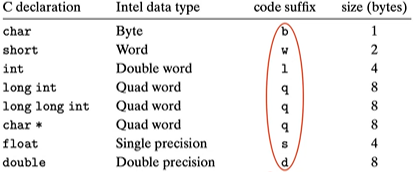
\includegraphics[scale = 0.5]{./figures/mechTypes}
\end{figure}
Note, there are no aggregate types like a list or array structure.Everything is just continuous bytes in memory.

\paragraph{Operations}
\begin{itemize}
        \item Transfer Data between Memory and Register - load data into register and save resister data into memory
        \item Perform arithmetic on register data
        \item Transfer control - unconditional jumps to or from procedures and conditional branches.
\end{itemize}

The Assembler translates Asm Code into Object code, which is in binary. This binary is nearly executable accept the linker must
do its namesake and resolves references between files like math (ie. -lm math). Some libraries are dynamically linked - this coccurs 
when the program begins execution.

\section*{Example}
This is a machine instruction example from C to Assembly to Machine code.
\begin{itemize}
        \item[\texttt{*dest = t}] store the value $t$ designated as  $dest$
        \item[\texttt{movq \%rax, (\%rbx)}] Move 8-byte value (aka Quad Word) to memory.\\
                $\%rax = t, \;\; \%rbx = dest, \;\; M[\%rbx] = \text{*}dest$\\
                Where $rax, rbx$ are in the register and  $M[rbx]$ is in memory
        \item[\texttt{0x40059e:48 89 03}] Three byte instruction stored at address $0x40059e$
\end{itemize}
\pagebreak


Looking at the full code from \texttt{objdump -d sumprogram} we can see the object code of a program:
\begin{figure}[h]
        \centering
        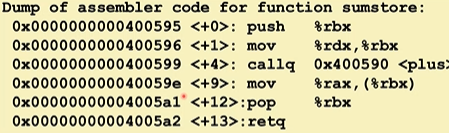
\includegraphics{./figures/objDump}
\end{figure}

The full list of the registers ($\%xy$) that can be used above are as follows:
 \begin{figure}[h]
         \centering
         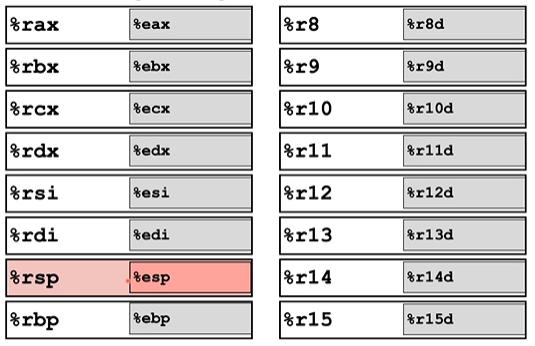
\includegraphics[scale = 0.7]{./figures/objReg}
\end{figure}

\section*{Moving Data}
In Assembly Code, use \texttt{movq\textit{ source }\textit{destination}}

The operand typed for the \texttt{movq} command are:
\begin{itemize}
        \item[\textbf{Immediate}] Constant integer data like \texttt{\$0x400, \$-53}
        \item[\textbf{Register}] One of 16 integer registers like \texttt{\%rax, \%r13}. However note that \texttt{\%rsp} is reserved for
                special use.
        \item[\textbf{Memory}] 8 consecutive bytes of memory at address given by register. for example, \texttt{\%rax}. 
                There are various `address modes' within Memory
\end{itemize}

Clearly there are many combinations of operands when using \texttt{movq}. They can be visualized like so:
\begin{figure}[h]
        \centering
        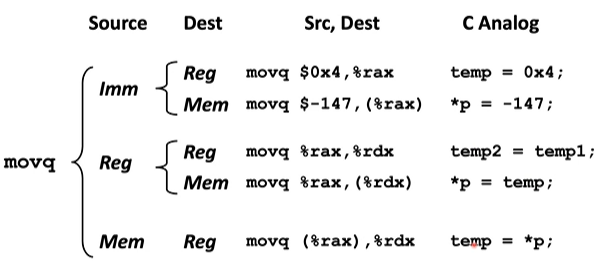
\includegraphics[scale = 0.7]{./figures/movqOperations}
\end{figure}

\subsection*{Simple Addressing Modes}
There are 2 types of Addressing modes when using movq.
\begin{itemize}
        \item[\textbf{Normal}] (R) Mem[Reg[R]]\\
                Register R specifies a memory address.\\
                \texttt{movq (\%rcx), \%rax}
        \item[\textbf{Displacement}] D(R) Mem[Reg[R]+D]\\
                Register R specifies start of memory region. The constant displacement D specifies offset.\\
                \texttt{movq 8(\%rbp), \%rdx}
\end{itemize}
Note: Registers start with a \%.
\begin{figure}
        \centering
        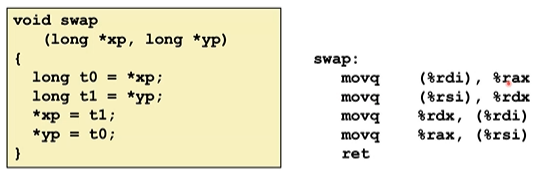
\includegraphics[scale = 0.6]{./figures/addressex1}
        
\end{figure}

\end{document}

